\documentclass[a4paper, 10pt]{letter}


% generowanie PDF, kolory, grafika...
\usepackage[pdftex,colorlinks=true,urlcolor=black,linkcolor=black]{hyperref}
\usepackage[pdftex,usenames]{color}
\usepackage[pdftex]{graphicx}


% zmiany domy¶lnego wygl±du dokumentu
\addtolength{\hoffset}{-2cm}
\addtolength{\textwidth}{4cm}
\addtolength{\voffset}{-1cm}
\addtolength{\textheight}{2cm}
%\setlength{\headwidth}{\textwidth}

% domy¶lne czcionki
\renewcommand\familydefault{\sfdefault}
%\renewcommand\sfdefault{phv}

\setlength{\columnseprule}{0.4pt} % pionowa czarna kreska miêdzy szpaltami
\newcommand{\inic}[1]{\dropping[0mm]{3}{#1\hspace{.5mm}}}

\frenchspacing
%\pagestyle{fancy}
%\fancyhf{}% czyszczê paginy


\usepackage[TS1,OT1,T1]{fontenc}
\usepackage[polish]{babel}
\usepackage[utf8]{inputenc}

\newcommand{\n}{Szymon Nieradka}

\newcommand{\from}{%
	\hspace{1cm}\n{} \\
	\hspace{1cm}Wilcza 69/23, Warszawa \\
	\hspace{1cm}Nr. dowodu: ARE238783 \\
	\hspace{1cm}Tel 693 373 068 \\
	\hspace{1cm}Email: szymon@nieradka.net
}

\begin{document}
\begin{letter}{\large{Referat Oskarżycieli Publicznych \\
I Oddział Terenowy \\
ul. Sołtyka 8/10 \\
Warszawa}}

\opening{{\large{Zgłoszenie wykroczenia \textit{231/2E}}}}

	W dniu 21 listopada 2017 roku o godzinie 14:00 byłem świadkiem pozostawienia
	samochodu Citroen nr rejestracyjny WW381WU na przejściu dla pieszych przy
	ulicy Poznańskiej 7 w Warszawie (róg ul. Poznańskiej i Wilczej). Pojazd
	zasłaniał przejście dla pieszych. Sytuacja jest widoczna na załączonych
	zdjęciach.

	Nie byłem świadkiem samego momentu parkowania oraz nie wiem jak długo
	pozostawał on w tym miejscu.

	Dane adresowe oraz kontaktowe zgłaszającego:
	\closing{\from{}}

	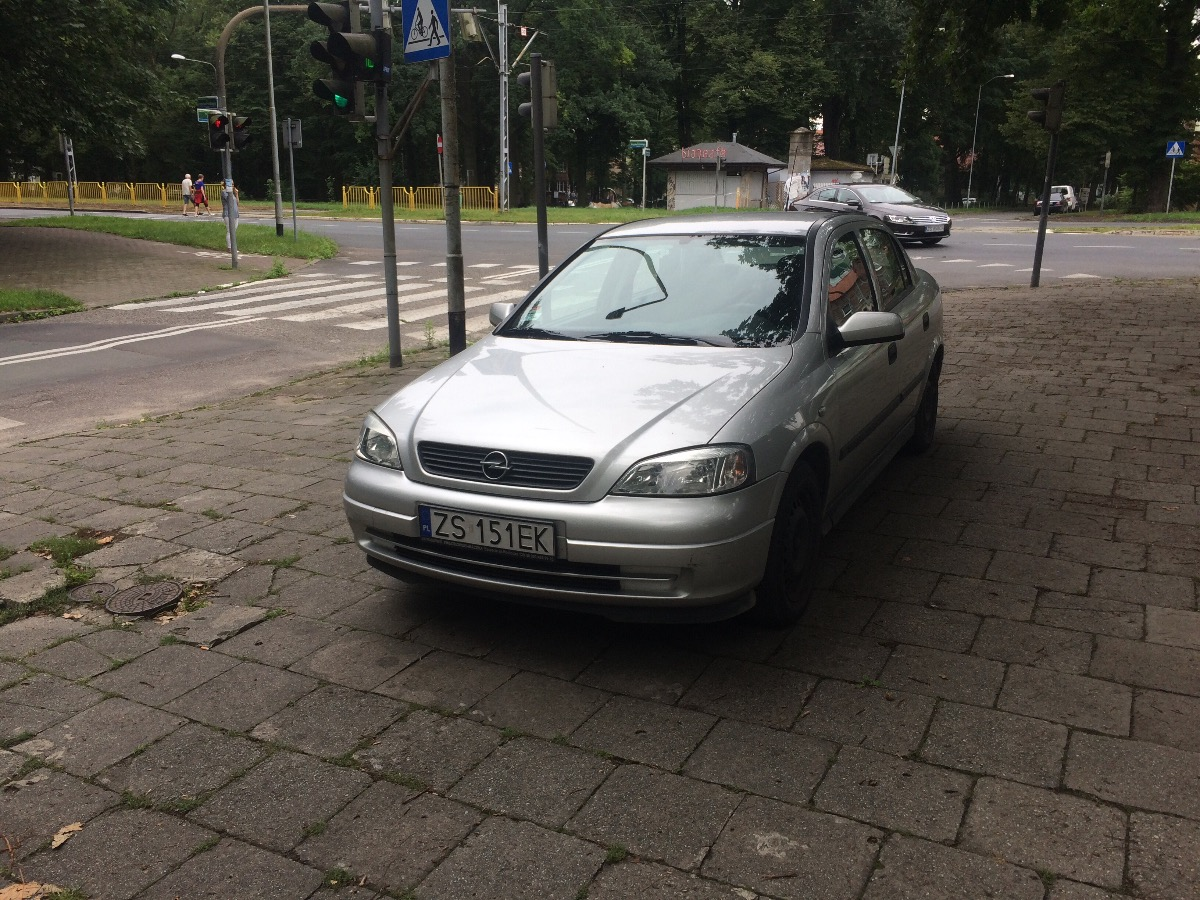
\includegraphics[width=0.5\textwidth]{5996f0cf6ea54.jpg}
	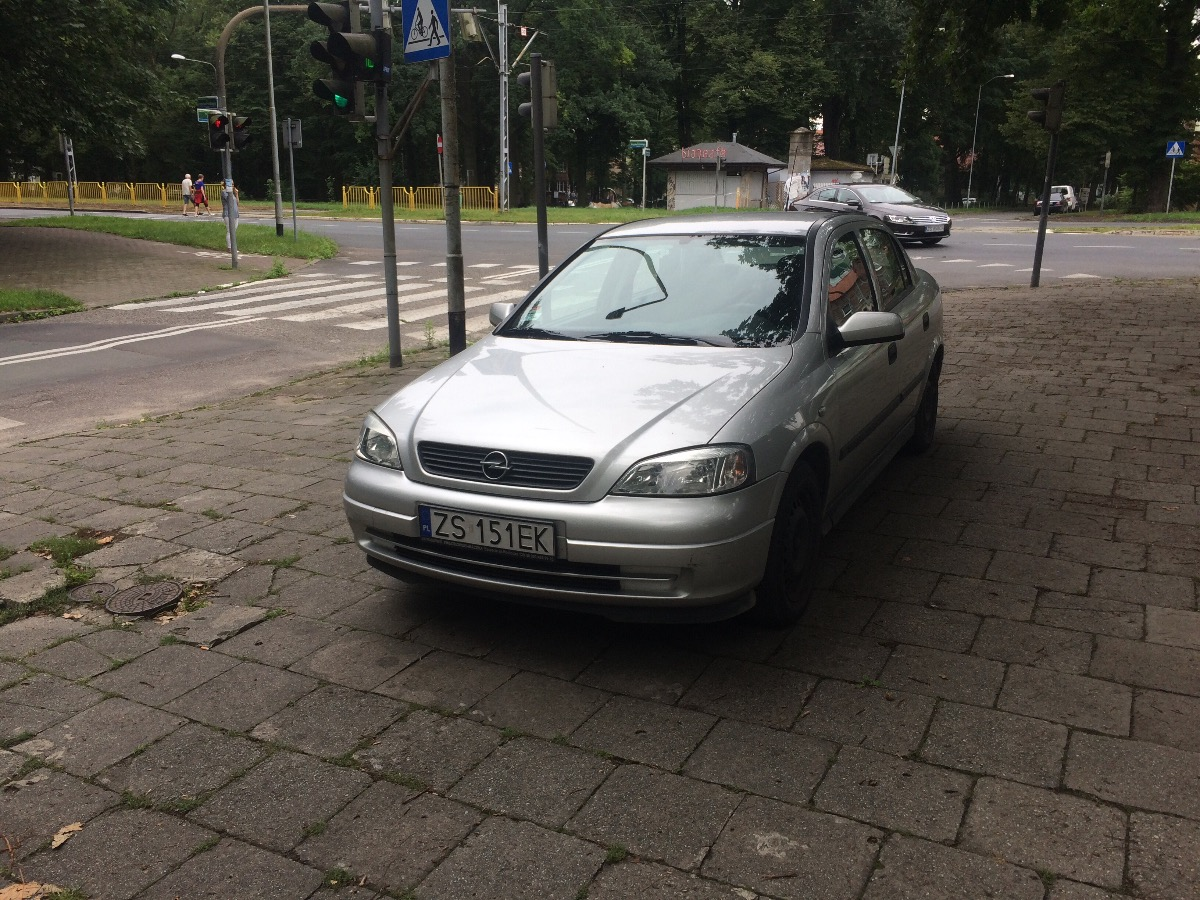
\includegraphics[width=0.5\textwidth]{5996f0cf6ea54.jpg}
\end{letter}
\end{document}
